\section{Results}\label{sec:results}

\maybeinput{tables/main_results.tex}

\textit{RQ1: gate pass rates.} Table~\ref{tab:main} reports every configuration. For the strongest model
(\BestModel), behavioural equivalence rises from \PlainEquiv\% with the plain prompt to \TrapEquiv\% with the
trap-aware prompt and \AgenticEquiv\% with the agent, against \RulesEquiv\% for the rule baseline; deployment
success rises from \PlainGOne\% to \AgenticGOne\%. The checklist is the significant ingredient: it adds \CheckEffect{} points of
case-level equivalence (95\% CI \CheckEffectCI; plain-only/trap-only correct \PlainTrapDisc, Holm-adjusted
$\PlainTrapP$), whereas repair adds \RepairEffect{} (\RepairEffectCI; $\TrapAgentP$). The repair loop ran in
\RepairShare\% of agentic runs; on these short cases it is a small, non-significant addition. The agent still
beats the rule baseline ($\RulesAgentP$). Size does not help without the checklist: with the plain prompt the
14B model outperforms both 32B variants. The 32B models translate near-literally, carrying ASE semantics
across whenever the code still compiles, and in a few runs split a procedure with \texttt{GO}
(\GoSplitShare\% of plain-prompt deployment failures)---plausibly prompted by the instruction to separate
batches with \texttt{GO}. With the checklist, the 32B models lead, though their intervals overlap the 14B
model's.

\textit{RQ2: the silent share.} Of plain-prompt translations from the strongest model that deployed,
\PlainSilentGivenCompile\% were behaviourally wrong. Overall, \PlainSilent\% of its plain runs and
\AgenticSilent\% of its agentic runs passed G1 and G2 yet failed G3. For the agent, \BestAgentSilentShare\%
of all remaining failures are silent: the gates removed every failure they can observe, and what is left is
exactly the class that only differential testing exposes.

\maybeinput{tables/observability.tex}

\textit{RQ3: what stays hard.} Table~\ref{tab:observability} splits equivalence by trap class, with a
counter-intuitive result. The agent scores \AgenticSilentClassEquiv\% on traps \emph{labelled} silent
(plain: \PlainSilentClassEquiv\%), because the checklist names them, but \AgenticCompileClassEquiv\% on
compile-visible traps (plain: \PlainCompileClassEquiv\%), where the \emph{repair} of a construct that will
not compile often produces code that compiles but behaves differently:
the GROUP BY extension is ``fixed'' by grouping or partitioning per row (C10, C28), a legacy right outer
join is rewritten with the wrong preserved table (C29), and unsigned types are narrowed to same-width
signed types that overflow on real values (C35, C36). In other words, fixing a loud error is a common
source of a quiet one.

\maybeinput{tables/failures.tex}

\textit{Error analysis.} Table~\ref{tab:failures} lists the cases that most often slipped past G1 and G2.
Two further patterns recur across models. First, surface rewriting can defeat lint while keeping the bug:
one model translated \texttt{mgr\_id = null} as \texttt{mgr\_id = convert(int, null)}, which passes the
\texttt{= NULL} rule and still returns no rows (C08). Second, error translation is fragile:
\texttt{raiserror (20001, 16, 1, ...)} raises SQL Server's built-in replication message 20001 rather than
the intended text, and \texttt{THROW} rejects ASE's user-error range outright (C05).

\IfFileExists{figures/category_g3.pdf}{%
\begin{figure}[t]\centering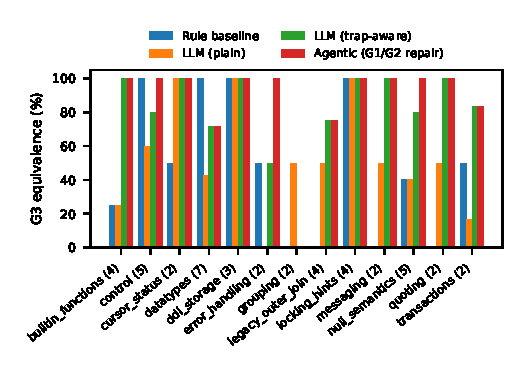
\includegraphics[width=\columnwidth]{figures/category_g3.pdf}
\caption{G3 equivalence by trap category for the strongest model.}\label{fig:cat}\end{figure}}{}

\textit{Held-out procedures.} On the \NumHeldout{} composite procedures (\HeldoutRuns{} graded runs), the
strongest model reaches \HeldoutPlainEquiv\% with the plain prompt, \HeldoutTrapEquiv\% with the checklist,
and \HeldoutAgenticEquiv\% with the agent (rule baseline: \HeldoutRulesEquiv\%). Deployment success is
\HeldoutTrapGOne\% for the trap-aware prompt and \HeldoutAgenticGOne\% for the agent, which repaired
\HeldoutRepairShare\% of these longer translations.
\note{After the held-out runs: one sentence on whether the checklist still helps on code it was not written
from, and whether repair matters more here than on single-trap cases.}

\textit{RQ4: size, quantization, and cost.} Fig.~\ref{fig:scaling} plots equivalence against mean latency
per case. The 4-bit and 8-bit 32B models reach the same agentic equivalence, while the 8-bit model is
slower, so on this hardware 4-bit quantization costs no measured accuracy. The 14B model trails slightly at lower latency,
and the second model family is weakest under every converter. Every configuration translates a case in seconds on a single
workstation.

\IfFileExists{figures/scaling.pdf}{%
\begin{figure}[t]\centering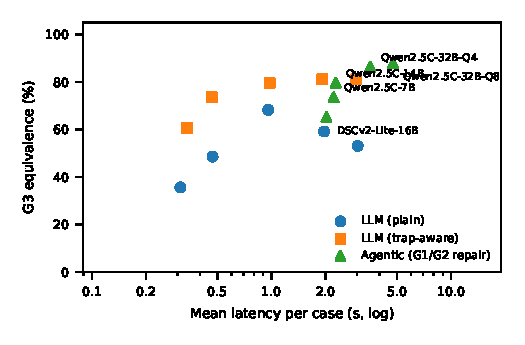
\includegraphics[width=\columnwidth]{figures/scaling.pdf}
\caption{Equivalence versus mean latency per case; labels mark agentic runs per model.}\label{fig:scaling}\end{figure}}{}

\maybeinput{tables/reconcile.tex}

\textit{RQ5: reconciliation.} Across injected single-row faults, row counts detect \RecRowcount\%, the
aggregate checksum \RecAggregate\%, and per-row hashing \RecRowhash\%, with no false positives on clean
trials (Table~\ref{tab:reconcile}). Row counts see only faults that change cardinality, so the content
faults typical of type-mapping errors---truncation, charset loss, rounding, precision loss---all pass a
count-only check. The aggregate checksum catches those but misses every swap of values between rows, which is
consistent with an order-insensitive, XOR-like combination of row checksums (the algorithm is not
documented). Only per-row hashing detects every fault.
